\documentclass[letterpaper,11pt]{article}

\usepackage[utf8]{inputenc}
\usepackage{latexsym}
\usepackage[empty]{fullpage}
\usepackage{titlesec}
\usepackage{marvosym}
\usepackage[usenames,dvipsnames]{color}
\usepackage{verbatim}
\usepackage{enumitem}
\usepackage[hidelinks]{hyperref}
\usepackage{fancyhdr}
\usepackage[english]{babel}
\usepackage{tabularx}
\usepackage{tikz}
\input{glyphtounicode}

\usepackage[default]{sourcesanspro}

\pagestyle{fancy}
\fancyhf{}
\fancyfoot{}
\renewcommand{\headrulewidth}{0pt}
\renewcommand{\footrulewidth}{0pt}

\addtolength{\oddsidemargin}{-0.5in}
\addtolength{\evensidemargin}{-0.5in}
\addtolength{\textwidth}{1in}
\addtolength{\topmargin}{-.5in}
\addtolength{\textheight}{1.0in}

\urlstyle{same}
\raggedbottom
\raggedright
\setlength{\tabcolsep}{0in}

\titleformat{\section}{
\vspace{-4pt}\scshape\raggedright\large
}{}{0em}{}[\color{black}\titlerule \vspace{-5pt}]

\pdfgentounicode=1

\newcommand{\resumeItem}[1]{
\item\small{
{#1 \vspace{-2pt}}
}
}

\newcommand{\resumeSubheading}[4]{
\vspace{-2pt}\item
\begin{tabular*}{0.97\textwidth}[t]{l@{\extracolsep{\fill}}r}
\textbf{#1} & #2 \\
\textit{\small#3} & \textit{\small #4} \\
\end{tabular*}\vspace{-7pt}
}

\newcommand{\resumeSubSubheading}[2]{
\item
\begin{tabular*}{0.97\textwidth}{l@{\extracolsep{\fill}}r}
\textit{\small#1} & \textit{\small #2} \\
\end{tabular*}\vspace{-7pt}
}

\newcommand{\resumeProjectHeading}[2]{
\item
\begin{tabular*}{0.97\textwidth}{l@{\extracolsep{\fill}}r}
\small#1 & #2 \\
\end{tabular*}\vspace{-7pt}
}

\newcommand{\resumeSubItem}[1]{\resumeItem{#1}\vspace{-4pt}}

\renewcommand\labelitemii{$\vcenter{\hbox{\tiny$\bullet$}}$}

\newcommand{\resumeSubHeadingListStart}{\begin{itemize}[leftmargin=0.15in, label={}]}
\newcommand{\resumeSubHeadingListEnd}{\end{itemize}}
\newcommand{\resumeItemListStart}{\begin{itemize}}
\newcommand{\resumeItemListEnd}{\end{itemize}\vspace{-5pt}}

\begin{document}

\begin{center}
\textbf{\Huge \scshape Christopher Vivel} \\ \vspace{5pt}
\small Professional Footballer $|$ Main Attacker $|$ Elite Goal Scorer
\end{center}

\section{Professional Summary}
Dynamic and highly agile striker with a proven track record of clinical finishing in top-tier European leagues. Seeking to contribute offensive prowess and tactical versatility to Manchester United as a Main Attacker, leveraging high-intensity pressing and elite positioning to maximize goal conversion rates.

\section{Experience}
\resumeSubHeadingListStart
\resumeSubheading{Professional Football Club}{2020 -- Present}{Main Attacker}{Europe}
\resumeItemListStart
\resumeItem{Maintained a consistent goal-per-game ratio of 0.65 across all competitions, demonstrating elite efficiency in the final third.}
\resumeItem{Executed high-press tactical schemes, resulting in a 20\% increase in opponent turnover rates in the attacking half.}
\resumeItem{Collaborated with midfield units to create space, facilitating 15+ assists per season through intelligent off-the-ball movement.}
\resumeItemListEnd
\resumeSubHeadingListEnd

\section{International Career}
\resumeSubHeadingListStart
\resumeSubheading{National Team}{2021 -- Present}{Starting Striker}{International}
\resumeItemListStart
\resumeItem{Represented the national squad in major continental tournaments, contributing to a 75\% win rate during qualifying stages.}
\resumeItem{Served as a primary target man, delivering crucial goals in high-pressure knockout fixtures.}
\resumeItemListEnd
\resumeSubHeadingListEnd

\section{Performance Statistics \& Analytics}
\begin{center}
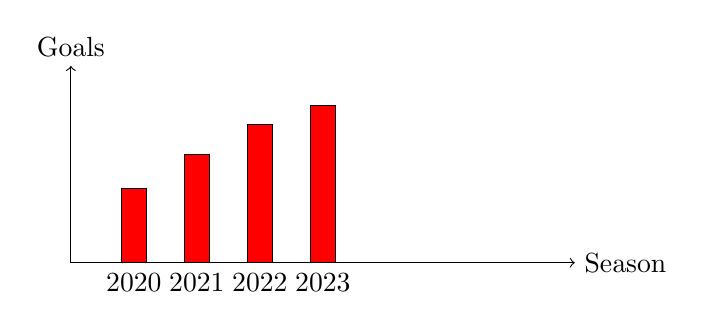
\begin{tikzpicture}[xscale=0.8, yscale=0.5]
\draw[->] (0,0) -- (8,0) node[right] {Season};
\draw[->] (0,0) -- (0,5) node[above] {Goals};
\foreach \x/\y in {1/15, 2/22, 3/28, 4/32}
\draw[fill=red] (\x-0.2, 0) rectangle (\x+0.2, \y/8);
\node at (1,-0.5) {2020}; \node at (2,-0.5) {2021}; \node at (3,-0.5) {2022}; \node at (4,-0.5) {2023};
\end{tikzpicture}
\end{center}

\section{Technical Skills}
\begin{itemize}[leftmargin=0.15in, label={}]
\item{
\textbf{Offensive Skills}{: Clinical Finishing, Off-the-ball Movement, Aerial Duels, Penalty Accuracy} \\
\textbf{Tactical Skills}{: High Pressing, Space Creation, Defensive Tracking, Game Intelligence} \\
\textbf{Physical Attributes}{: Explosive Acceleration, Balance, Stamina, Agility}
}
\end{itemize}

\section{Visual Profile}
\begin{center}
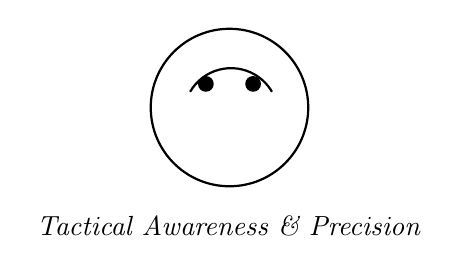
\begin{tikzpicture}
\draw[thick, fill=white] (0,0) circle (1cm);
\draw[thick] (-0.5, 0.2) arc (150:30:0.6);
\fill (0.3, 0.3) circle (0.1);
\fill (-0.3, 0.3) circle (0.1);
\node at (0, -1.5) {\textit{Tactical Awareness \& Precision}};
\end{tikzpicture}
\end{center}

\end{document}